%% Template pour rapport de stage du master AIC (Apprentissage,
%% Information et Contenu), Université Paris-Saclay
%% Template d'origine : 
%% Copyright (C) 2008 Johan Oudinet <oudinet@lri.fr>
%%  
%% Permission is granted to make and distribute verbatim copies of
%% this manual provided the copyright notice and this permission notice
%% are preserved on all copies.
%%  
%% Permission is granted to process this file through TeX and print the
%% results, provided the printed document carries copying permission
%% notice identical to this one except for the removal of this paragraph
%% (this paragraph not being relevant to the printed manual).
%%  
%% Permission is granted to copy and distribute modified versions of this
%% manual under the conditions for verbatim copying, provided that the
%% entire resulting derived work is distributed under the terms of a 
%% permission notice identical to this one.
%%  
%% Permission is granted to copy and distribute translations of this manual
%% into another language, under the above conditions for modified versions,
%% except that this permission notice may be stated in a translation
%% approved by the Free Software Foundation
%%  

\documentclass[oneside]{memoir}
\let\STARTCODE\relax 
\let\STOPCODE\relax 
\STARTCODE
\usepackage{color,calc,graphicx,soul}
\definecolor{nicered}{rgb}{.647,.129,.149} \makeatletter
\newlength\dlf@normtxtw \setlength\dlf@normtxtw{\textwidth}
\def\myhelvetfont{\def\sfdefault{mdput}} \newsavebox{\feline@chapter}
\newcommand\feline@chapter@marker[1][4cm]{%
  \sbox\feline@chapter{%
    \resizebox{!}{#1}{\fboxsep=1pt%
      \colorbox{nicered}{\color{white}\bfseries\sffamily\thechapter}%
    }}%
  \rotatebox{90}{%
    \resizebox{%
      \heightof{\usebox{\feline@chapter}}+\depthof{\usebox{\feline@chapter}}}%
    {!}{\scshape\so\@chapapp}}\quad%
  \raisebox{\depthof{\usebox{\feline@chapter}}}{\usebox{\feline@chapter}}%
} \newcommand\feline@chm[1][4cm]{%
  \sbox\feline@chapter{\feline@chapter@marker[#1]}%
  \makebox[0pt][l]{% aka \rlap
    \makebox[1cm][r]{\usebox\feline@chapter}%
  }} \makechapterstyle{daleif1}{
%   \setlength{\beforechapskip}{0pt}
%   \setlength{\midchapskip}{0pt}
  \setlength{\afterchapskip}{10pt}
%   \setlength{\chapindent}{0pt}
  \renewcommand{\insertchapterspace}{}
  \renewcommand\chapnamefont{\normalfont\Large\scshape\raggedleft\so}
  \renewcommand\chaptitlefont{\normalfont\huge\bfseries\scshape\color{nicered}}
  \renewcommand\chapternamenum{} 
  \renewcommand\printchaptername{}
  \renewcommand\printchapternum{\vspace{-5.5cm}\null\hfill\feline@chm[2.5cm]\par}
  \renewcommand\afterchapternum{\par\vskip\midchapskip}
  \renewcommand\printchaptertitle[1]{\chaptitlefont\raggedleft
    ##1\par}
  \renewcommand\printchapternonum{\vspace{-3.5cm}}
 %  \renewcommand{\insertchapterspace}{}
}


\makeatother
\chapterstyle{daleif1}
\STOPCODE




\usepackage[latin1]{inputenc}
\usepackage{epsfig}
\usepackage{acronym}
\usepackage{amssymb}
\usepackage{amsmath}
\usepackage{amsfonts}
\usepackage{pgf}
\usepackage{tikz}
\usepackage{setspace}%
\usepackage{hhline}
\usepackage[colorlinks]{hyperref}
\usepackage[all]{hypcap}
\usepackage{algorithm, algorithmic}
\usepackage[french]{babel}
\usetikzlibrary{shapes,arrows,automata,backgrounds}
\usepackage{wrapfig}
\usepackage{microtype}
\usepackage{multicol}
% \usepackage[T1]{fontenc}

% francisation des algorithmes
\renewcommand{\sectionmark}[1]{}
\renewcommand{\algorithmicrequire} {\textbf{\textsc{Entrées:}}}
\renewcommand{\algorithmicensure}  {\textbf{\textsc{Sorties:}}}
\renewcommand{\algorithmicwhile}   {\textbf{tantque}}
\renewcommand{\algorithmicdo}      {\textbf{faire}}
\renewcommand{\algorithmicendwhile}{\textbf{fin tantque}}
\renewcommand{\algorithmicend}     {\textbf{fin}}
\renewcommand{\algorithmicif}      {\textbf{si}}
\renewcommand{\algorithmicendif}   {\textbf{finsi}}
\renewcommand{\algorithmicelse}    {\textbf{sinon}}
\renewcommand{\algorithmicthen}    {\textbf{alors}}
\renewcommand{\algorithmicfor}     {\textbf{pour}}
\renewcommand{\algorithmicforall}  {\textbf{pour tout}}
\renewcommand{\algorithmicdo}      {\textbf{faire}}
\renewcommand{\algorithmicendfor}  {\textbf{fin pour}}
\renewcommand{\algorithmicloop}    {\textbf{boucler}}
\renewcommand{\algorithmicendloop} {\textbf{fin boucle}}
\renewcommand{\algorithmicrepeat}  {\textbf{répéter}}
\renewcommand{\algorithmicuntil}   {\textbf{jusqu'à}}

\floatname{algorithm}{Algorithme}


%
% Definir les termes francais 
%
  \gdef\@dedicace{D\'edicace}
  \gdef\@remerciements{Remerciements}
  \def\prefacename{Avant-propos}
  \def\refname{R\'ef\'erences}
  \gdef\@resume{R\'esum\'e}
  \gdef\@notation{Notation}
   \gdef\@abbreviation{Liste des Sigles}
  \gdef\abstractname{Abstract}
  \def\bibname{R\'ef\'erences}
  \gdef\@introduction{Introduction}
  \def\chaptername{Chapitre}
  \gdef\@conclusion{Conclusion}
  \def\appendixname{Annexe}
  \gdef\@tabledesmatieres{Table des mati\`eres}
  \gdef\@listedesfigures{Liste des figures}
  \gdef\@listedeslistings{Liste des codes source}
  \gdef\@listedestableaux{Liste des tableaux}
  \gdef\@listedesannexes{Liste des annexes}
  \def\indexname{Index}
  \def\figurename{Figure}
  \def\tablename{Tableau}
  \def\partname{Partie}
  \def\ccname{Copie \`a}
  \def\pagename{Page}
\def\today{\ifnum\day=1\relax 1\/$^{\rm er}$\else
  \number\day\fi \space\ifcase\month\or
  janvier\or f\'evrier\or mars\or avril\or mai\or juin\or
  juillet\or ao\^ut\or septembre\or octobre\or novembre\or
  d\'ecembre\fi
  \space\number\year} 

% Malheureusement, il y a un bogue dans Babel qui fait que
% figurename, tablename, etc. se réinitialise toujours à la valeur par
% défaut. Plutôt qu'avoir Figure et Tableau, en Français, on a
% Fig et Tab, à moins de recopier.
\def\captionsfrench{
   \def\refname{R\'ef\'erences}%
   \def\abstractname{R\'esum\'e}%
   \def\bibname{Bibliographie}%
   \def\prefacename{Avant-propos}%
   \def\chaptername{Chapitre}%
   \def\appendixname{Annexe}%
   \def\contentsname{Table des mati\`eres}%
   \def\listfigurename{Liste des figures}%
   \def\listtablename{Liste des tableaux}%
   \def\indexname{Index}%
   \def\figurename{Figure}%
   \def\tablename{Tableau}%
   \def\CaptionSeparator{\space\textendash\space}%
   \def\partname{\protect\@Fpt partie}%
   \def\@Fpt{{\ifcase\value{part}\or Premi\`ere\or Deuxi\`eme\or
   Troisi\`eme\or Quatri\`eme\or Cinqui\`eme\or Sixi\`eme\or
   Septi\`eme\or Huiti\`eme\or Neuvi\`eme\or Dixi\`eme\or Onzi\`eme\or
   Douzi\`eme\or Treizi\`eme\or Quatorzi\`eme\or Quinzi\`eme\or
   Seizi\`eme\or Dix-septi\`eme\or Dix-huiti\`eme\or Dix-neuvi\`eme\or
   Vingti\`eme\fi}\space\def\thepart{}}%
   \def\pagename{page}%
   \def\seename{{\emph{voir}}}%
   \def\alsoname{{\emph{voir aussi}}}%
   \def\enclname{P.~J. }%
   \def\ccname{Copie \`a }%
   \def\headtoname{}%
   \def\proofname{D\'emonstration}% for AMS-\LaTeX
   \def\glossaryname{Glossaire}%
}


%% Page layout
\setlength{\oddsidemargin}{1cm}
\setlength{\evensidemargin}{1.5cm}
\setlength{\topmargin}{0cm}
\setlength{\textheight}{21cm}
\setlength{\textwidth}{15cm}

% \setlength{\beforeschapskip}{-2cm}

\newcommand{\HRule}{\rule{\linewidth}{0.5mm}}
\DeclareMathOperator*{\argmin}{arg\,min}

\begin{document}

\begin{titlingpage}
 
\begin{center}
 
%%%%%%%%%%%%%%%%%%%%%%%%%%%%%%%%%%%%%%%%%%%%%%%%%%%%%%%%%%%%%%%%%%%%%%%%%
% LOGOS: 
% 

\includegraphics[height=2cm]{logos/upsay.pdf} \hfill % Paris-Saclay: Don't remove !

\includegraphics[height=2cm]{logos/ups.png} % Your school inside Paris-Saclay
\\[1.5cm]


%%%%%%%%%%%%%%%%%%%%%%%%%%%%%%%%%%%%%%%%%%%%%%%%%%%%%%%%%%%%%%%%%%%%%%%%%
% Your specific logos (labs, companies, .... )
\begin{minipage}{0.2\textwidth}
  \begin{flushright}
    
\includegraphics[width=0.6\textwidth]{logos/limsi.png}
  \end{flushright}
\end{minipage}
\begin{minipage}{0.2\textwidth}
  \begin{flushright}
    
\includegraphics[width=0.5\textwidth]{logos/lri.png}
  \end{flushright}
\end{minipage}


\vspace{2cm} 
\textsc{\Large Stage de Master 2 Recherche en Informatique}\\[0.5cm]
 
 
% Title
\HRule \\[0.4cm]
{ \huge \bfseries Introducing prior knowledge in the loss function in order to do segmentation of medical images}\\[0.4cm]
 
\HRule \\[1.5cm]
 
% Author and supervisor
\begin{minipage}{0.4\textwidth}
\begin{flushleft} \large
\emph{Auteur :}\\
Prénom \textsc{Nom}
\end{flushleft}
\end{minipage}
\begin{minipage}{0.4\textwidth}
\begin{flushright} \large
\emph{Responsable de stage :} \\
Dr. Prénom \textsc{Nom}
\end{flushright}
\end{minipage}
\vfill
\emph{Organisme d'accueil : }\\
Laboratoire Truc

 
\vfill


 
% Bottom of the page
{Secrétariat - tél : 01 69 15 81 58\\
courrier électronique : alexandre.verrecchia@u-psud.fr\\
} 
\end{center}
 
\end{titlingpage}

\newcommand{\Loss}{\mathcal{L}}

\pagenumbering{roman}

\tableofcontents

\newpage
\thispagestyle{empty}%
\newpage

\chapter*{Résumé}

Post hoc impie perpetratum quod in aliis quoque iam timebatur, tamquam
licentia crudelitati indulta per suspicionum nebulas aestimati quidam
noxii damnabantur. quorum pars necati, alii puniti bonorum multatione
actique laribus suis extorres nullo sibi relicto praeter querelas et
lacrimas, stipe conlaticia victitabant, et civili iustoque imperio ad
voluntatem converso cruentam, claudebantur opulentae domus et
clarae~\cite{ammianius42}.

\section*{Mots clefs}
Post, impie, aliis, multatione, domus.

\pagebreak

\pagenumbering{arabic}
\setcounter{page}{1}

%% Copyright (C) 2008 Johan Oudinet <oudinet@lri.fr>
%%  
%% Permission is granted to make and distribute verbatim copies of
%% this manual provided the copyright notice and this permission notice
%% are preserved on all copies.
%%  
%% Permission is granted to process this file through TeX and print the
%% results, provided the printed document carries copying permission
%% notice identical to this one except for the removal of this paragraph
%% (this paragraph not being relevant to the printed manual).
%%  
%% Permission is granted to copy and distribute modified versions of this
%% manual under the conditions for verbatim copying, provided that the
%% entire resulting derived work is distributed under the terms of a 
%% permission notice identical to this one.
%%  
%% Permission is granted to copy and distribute translations of this manual
%% into another language, under the above conditions for modified versions,
%% except that this permission notice may be stated in a translation
%% approved by the Free Software Foundation
%%  
\chapter{Introduction}
\label{sec:intro}

Post emensos insuperabilis expeditionis eventus languentibus partium
animis, quas periculorum varietas fregerat et laborum, nondum tubarum
cessante clangore vel milite locato per stationes hibernas, fortunae
saevientis procellae tempestates alias rebus infudere communibus per
multa illa et dira facinora Caesaris Galli, qui ex squalore imo
miseriarum in aetatis adultae primitiis ad principale culmen insperato
saltu provectus ultra terminos potestatis delatae procurrens
asperitate nimia cuncta foedabat. propinquitate enim regiae stirpis
gentilitateque etiam tum Constantini nominis efferebatur in fastus, si
plus valuisset, ausurus hostilia in auctorem suae felicitatis, ut
videbatur.

\section{Eo adducta re per Isauriam}
\label{sec:isauriam}

Eo adducta re per Isauriam, rege Persarum bellis finitimis inligato
repellenteque a conlimitiis suis ferocissimas gentes, quae mente
quadam versabili hostiliter eum saepe incessunt et in nos arma
moventem aliquotiens iuvant, Nohodares quidam nomine e numero
optimatum, incursare Mesopotamiam quotiens copia dederit ordinatus,
explorabat nostra sollicite, si repperisset usquam locum vi subita
perrupturus.

Batnae municipium in Anthemusia conditum Macedonum manu priscorum ab
Euphrate flumine brevi spatio disparatur, refertum mercatoribus
opulentis, ubi annua sollemnitate prope Septembris initium mensis ad
nundinas magna promiscuae fortunae convenit multitudo ad commercanda
quae Indi mittunt et Seres aliaque plurima vehi terra marique
consueta.

%%% Local Variables: 
%%% mode: latex
%%% TeX-master: "rapportM2R"
%%% End: 


\chapter{Presentation of the laboratory}

Cuius acerbitati uxor grave accesserat incentivum, germanitate Augusti
turgida supra modum, quam Hannibaliano regi fratris filio antehac
Constantinus iunxerat pater, Megaera quaedam mortalis, inflammatrix
saevientis adsidua, humani cruoris avida nihil mitius quam maritus;
qui paulatim eruditiores facti processu temporis ad nocendum per
clandestinos versutosque rumigerulos conpertis leviter addere quaedam
male suetos falsa et placentia sibi discentes, adfectati regni vel
artium nefandarum calumnias insontibus adfligebant.


\chapter{Relative works}

\subsection{Fully convolutional Networks for semantic segmentation \cite{Long_2015_CVPR}}
	On this paper \cite{Long_2015_CVPR} the authors show us how to train a convolutional neural network(CNN0) end-to-end pixel-to-pixel to do semantic segmentation. The method proposed allow us to use Convolutional Neural Network to segment an image and then to identify precisely a subpart of an image. We call that semantic segmentation.
    
    The difference with a regular CNN is instead of classifying images, we classify each pixel of each images. So the output of a CNN, must be of the same size as the image input.
    
    The authors explain how to transform any regular CNN in a fully CNN but also propose different fully CNN architecture.
    
    Firstly, to transform a classifier CNN into a fully CNN, we just have to transform all the fully connected layers into convolutional layers. Indeed 
    
    The main idea is to transform all the fullly connected layers into convolutional layers. With that we can upsample the input of the last hidden layer in order to have a heatmap as an input. Using this method we can classify each pixel of the image and then have a segmentation as output. 
    
    \begin{figure}
    	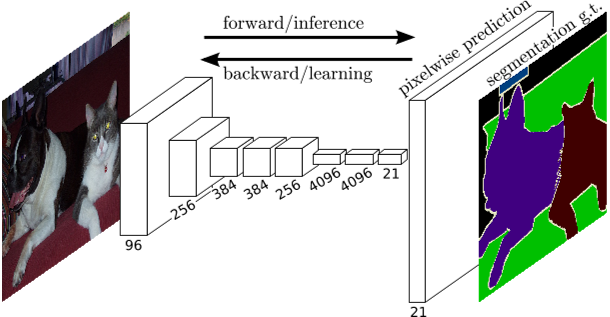
\includegraphics[width=0.49\linewidth]{images/fullCNN}
        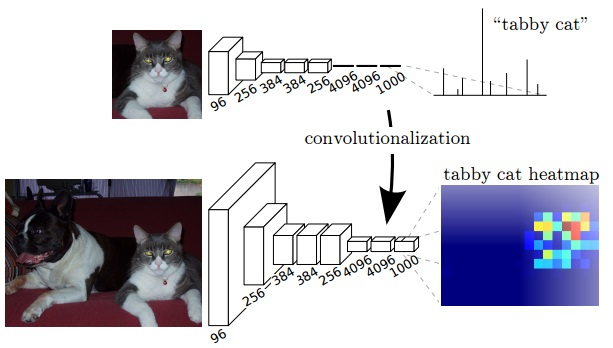
\includegraphics[width=0.49\linewidth]{images/FCN_heatmap}
        
        \caption{Fully CNN can learn to make prediction pixel-per-pixel for semantic segmentation}
        \label{fullCNN}
    \end{figure}
    
    The main difference between a fully CNN and a regular CNN, is that there is no fully connected layers in a fully CNN. So in every layer, we learn filters. 
    
     The number of kernels for every convolution layer equals the product of layers outputs to the number of input images.
    
    
end-to-end\\
receptive field : parameter, filter size. Region in which the neuron is connected\\
VGG net, GoogLeNet\\
Fully convolutional networks\\
skip architecure\\

mean IU(Intersection over union) segmentation : true positive / (true positive + false positive + false negative) \\


\subsection{Topology Aware Fully Convolutional Networks For Histology Gland Segmentation\cite{FCN_Gland_Segmentation}}
	
    We just saw how to train a CNN end-to-end in order to segment an image. The main disadvantage of using CNN with cross-entropy loss instead of using other methods is the fact that CNN does not have any prior knowledge about the dataset. He's just trying to solve an optimization problem in the same way that he'll solve it for any other dataset. 
    But introducing prior knowledge on a CNN, is not something impossible. One way to do it is to introduce prior knowledge in the loss function. 
    
    The paper \cite{FCN_Gland_Segmentation} propose different loss function which introduce prior knowledge in order to learn more efficiently the segmentation.
	
    They applied their methods for Histology Gland Segmentation. Given an input image, the goal is to identify the 3 different region : the background, the boundary around the gland, the inside glandular lumen.
    
     \begin{figure}
    	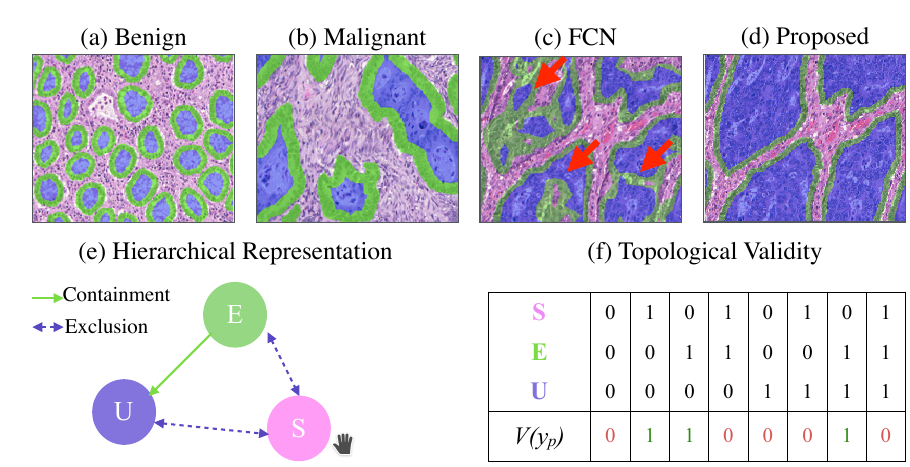
\includegraphics[width=\linewidth]{images/multiRegionGlandRepresentation}
        \label{MultiRegionGlandRepresentation}
        \caption{Multi region gland representation}
    \end{figure}
    
    Instead of using a Fully Convolutional Network per-pixel loss (cross entropy) : 
    
    \begin{center}
      \begin{align}
          \theta^* = \argmin_\theta \sum_{n=1}^N \Loss(x^{(n)};\theta) \\
          \Loss(x^{(n)};\theta) = \sum_{p\in\Omega}\sum_{r=1}^L -y_p^r log P(y_p^r = 1 | x_p; \theta)\\
          P(y_p^r = 1 | x_p; \theta) = \frac{exp(a_r(x_p}{\sum_{k=1}^L exp(a_k(x_p))}
      \end{align}
    \end{center}
    
    , they introduced hierarchical relations between region labels. Therefore, the loss function to optimize became : 
    \begin{align*}
    	\theta^* = \argmin_\theta \sum_{n=1}^N \alpha_1 \Loss_T(x^{(n)}; \theta) + \alpha_2 \Loss_S(x^{(n)}; \theta);
    \end{align*}
    
    Where $\Loss_T$ and $\Loss_S$ refer, in order, to the pixel-level loss functions that encode the topological relations betweens labels and the smoothness constraints. $\alpha_1$ and $\alpha_2$ are user-defined weights used to balance the contribution of each prior.
    
    $\Loss_T$ must be defined such that the network is trained, not only to penalize incorrect label assignment but also to penalize incorrect label hierarchy. For example, if we want a region U, to be contained in a region E, we want of course $P(y_p^U=1)$ to be high, but we also want $P(y_p^E=1)$ and $P(y_p^S=1)$ to be high (S is the background, cf figure \ref{MultiRegionGlandRepresentation}). That's why they defined the following unary loss : 
    \begin{align}
    	P(y_p | x_p; \theta) = 1/Z * \prod_{r=1}^L exp(a_r(x_p)) x y_p^r * V(y_p), Z =\sum_{r=1}^L P(y_p^r | x_p; \theta) 
    \end{align}
    
    
    
    
    
	

%% Copyright (C) 2008 Johan Oudinet <oudinet@lri.fr>
%%  
%% Permission is granted to make and distribute verbatim copies of
%% this manual provided the copyright notice and this permission notice
%% are preserved on all copies.
%%  
%% Permission is granted to process this file through TeX and print the
%% results, provided the printed document carries copying permission
%% notice identical to this one except for the removal of this paragraph
%% (this paragraph not being relevant to the printed manual).
%%  
%% Permission is granted to copy and distribute modified versions of this
%% manual under the conditions for verbatim copying, provided that the
%% entire resulting derived work is distributed under the terms of a 
%% permission notice identical to this one.
%%  
%% Permission is granted to copy and distribute translations of this manual
%% into another language, under the above conditions for modified versions,
%% except that this permission notice may be stated in a translation
%% approved by the Free Software Foundation
%%  
\chapter{Conclusion et perspectives}

Cuius acerbitati uxor grave accesserat incentivum, germanitate Augusti
turgida supra modum, quam Hannibaliano regi fratris filio antehac
Constantinus iunxerat pater, Megaera quaedam mortalis, inflammatrix
saevientis adsidua, humani cruoris avida nihil mitius quam maritus;
qui paulatim eruditiores facti processu temporis ad nocendum per
clandestinos versutosque rumigerulos conpertis leviter addere quaedam
male suetos falsa et placentia sibi discentes, adfectati regni vel
artium nefandarum calumnias insontibus adfligebant.

%%% Local Variables: 
%%% mode: latex
%%% TeX-master: "rapportM2R"
%%% End: 


\chapter*{Remerciements}
Saraceni tamen nec amici nobis umquam nec hostes optandi, ultro
citroque discursantes quicquid inveniri poterat momento temporis parvi
vastabant milvorum rapacium similes, qui si praedam dispexerint
celsius, volatu rapiunt celeri, aut nisi impetraverint, non
inmorantur.

\bibliographystyle{plain}
\bibliography{rapportM2R}

\appendix

% \input{appendixA}

\end{document}


%%% Local Variables: 
%%% mode: latex
%%% TeX-master: "rapportM2R"
%%% End: 
